% 
%            ,,                                        
%          `7MM            _.o9                                
%            MM                                             
%  ,6"Yb.    MM  ,p6"bo   ,6"Yb.  M"""MMV  ,6"Yb.  `7Mb,od8 
% 8)   MM    MM 6M'  OO  8)   MM  '  AMV  8)   MM    MM' "' 
%  ,pm9MM    MM 8M        ,pm9MM    AMV    ,pm9MM    MM     
% 8M   MM    MM YM.    , 8M   MM   AMV  , 8M   MM    MM     
% `Moo9^Yo..JMML.YMbmd'  `Moo9^Yo.AMMmmmM `Moo9^Yo..JMML.   
% 
% 
% Free, Open-Source Thesis template for LaTeX
% https://github.com/dpmj/alcazar


%%%%%%%%%%%%%%%%%%%%%%%%%%%%%%%%%%%%%%%%%%%%%%%%%%%%%%%%%%%%%%%%%%%%%%%%%%%%%%%%%%%%%%%%%%%%%%%%%
% PREAMBLE

\documentclass[twoside, openright, 11pt]{report}


% Variables

% Title for the title page 
\newcommand{\thesisTitle}{Alcázar: a free and open-source {\LaTeX} template for academic works, for nerd grown-up kids who do boring stuff such as theses with endless titles}
% Title for the pages' heading 
\newcommand{\thesisTitleShort}{Alcázar: a free and open-source {\LaTeX} template for academic works}

\newcommand{\thesisType}{Master's Thesis}  % Bachelor's Thesis, Master's Thesis, PhD Thesis...
\newcommand{\thesisDegree}{Master's Degree}  % Bachelor's Degree, Master's Degree, PhD...
\newcommand{\thesisArea}{Telecommunications Engineering}  % Area of knowledge

\newcommand{\thesisAuthor}{Name of the author of the thesis}
\newcommand{\thesisTutor}{Name of the supervisor of the thesis}  

\newcommand{\thesisYear}{2077}  % Date of the thesis' submission or defense 
\newcommand{\thesisMonth}{June}
\newcommand{\thesisDate}{{\thesisMonth} {\thesisYear}}
\newcommand{\thesisAcademicCourse}{2076/2077}  % During which academic year(s) was the thesis developed

\newcommand{\thesisSchool}{Universitat Politècnica de València}
\newcommand{\thesisAddress}{Camí de Vera, s/n, 46022 València, Valencia, Spain}
\newcommand{\thesisDepartment}{Department of Electronic Engineering}

\newcommand{\thesisKeywords}{Keyword 1, Keyword 2, Keyword 3, Keyword 4, Keyword 4, Keyword 5, Keyword 6, Keyword 7, Keyword 8, Keyword 9, Keyword 10, Keyword N}  
% For the abstract and indexing



% Import document style
\usepackage{style/alcazar}

% \usepackage{multibib}
% \newcites{latex}{Publications}


%%%%%%%%%%%%%%%%%%%%%%%%%%%%%%%%%%%%%%%%%%%%%%%%%%%%%%%%%%%%%%%%%%%%%%%%%%%%%%%%%%%%%%%%%%%%%%
% BEGIN DOCUMENT

\begin{document}

% Titlepage, license, about, abstract, keywords, publications, acknowledgements, dedication and tables of contents
% 
%            ,,                                        
%          `7MM            _.o9                                
%            MM                                             
%  ,6"Yb.    MM  ,p6"bo   ,6"Yb.  M"""MMV  ,6"Yb.  `7Mb,od8 
% 8)   MM    MM 6M'  OO  8)   MM  '  AMV  8)   MM    MM' "' 
%  ,pm9MM    MM 8M        ,pm9MM    AMV    ,pm9MM    MM     
% 8M   MM    MM YM.    , 8M   MM   AMV  , 8M   MM    MM     
% `Moo9^Yo..JMML.YMbmd'  `Moo9^Yo.AMMmmmM `Moo9^Yo..JMML.   
% 
% 
% Free and Open-Source template for academic works
% https://github.com/dpmj/alcazar



% Title page
% 
%            ,,                                        
%          `7MM            _.o9                                
%            MM                                             
%  ,6"Yb.    MM  ,p6"bo   ,6"Yb.  M"""MMV  ,6"Yb.  `7Mb,od8 
% 8)   MM    MM 6M'  OO  8)   MM  '  AMV  8)   MM    MM' "' 
%  ,pm9MM    MM 8M        ,pm9MM    AMV    ,pm9MM    MM     
% 8M   MM    MM YM.    , 8M   MM   AMV  , 8M   MM    MM     
% `Moo9^Yo..JMML.YMbmd'  `Moo9^Yo.AMMmmmM `Moo9^Yo..JMML.   
% 
% 
% Free and Open-Source template for academic works
% https://github.com/dpmj/alcazar


% ------------------------------------------------------------------------------
% Title page

\thispagestyle{empty}

\pagenumbering{roman}
\setcounter{page}{1}


\newgeometry{
    left    = 3.0cm,
    right   = 3.0cm,
    top     = 3.5cm,
    bottom  = 3.5cm
}


\begin{center}
    
\includegraphics[height=15mm]{opening/resources/logos/logo_upv.pdf}
    \hfill
    
\includegraphics[height=15mm]{opening/resources/logos/logo_upv_telcom.pdf}
\end{center}

\vspace*{30mm}

\begin{center}
    \textbf{\large \textsc{{\thesisDegree} in}}\\
    \textbf{\large \textsc{\thesisArea}}
\end{center}

\vspace*{0mm}

\begin{center}
    \textbf{\large \thesisType}
\end{center}

\vspace*{10mm}

\begin{center}
    \setstretch{1.7}
    \textbf{{\LARGE {}``\thesisTitle''}}\\
\end{center}

\vspace*{15mm}

\begin{center}
    {\large \textsc{Academic course:} \thesisAcademicCourse}
\end{center}

\vspace*{15mm}

\begin{center}
    AUTHOR:
    \par
    \textbf{{\large \thesisAuthor}}
\end{center}

\begin{center}
    TUTOR:
    \par
    \textbf{{\large \thesisTutor}}
\end{center}

\begin{center}
    \vspace*{1mm}
    {\large \thesisDepartment}
\end{center}

\newpage
\thispagestyle{empty}
\restoregeometry


% License
% 
%            ,,                                        
%          `7MM            _.o9                                
%            MM                                             
%  ,6"Yb.    MM  ,p6"bo   ,6"Yb.  M"""MMV  ,6"Yb.  `7Mb,od8 
% 8)   MM    MM 6M'  OO  8)   MM  '  AMV  8)   MM    MM' "' 
%  ,pm9MM    MM 8M        ,pm9MM    AMV    ,pm9MM    MM     
% 8M   MM    MM YM.    , 8M   MM   AMV  , 8M   MM    MM     
% `Moo9^Yo..JMML.YMbmd'  `Moo9^Yo.AMMmmmM `Moo9^Yo..JMML.   
% 
% 
% Free and Open-Source template for academic works
% https://github.com/dpmj/alcazar


%%%%%%%%%%%%%%%%%%%%%%%%%%%%%%%%%%%%%%%%%%%%%%%%%%%%%%%%%%%%%%%%%%%%%%%%%%%%%%%%%%%%%%%%%%%%
% LICENSE

\newpage
\thispagestyle{empty}

\vspace*{\fill}

\begingroup

    \setlength\tabcolsep{0pt}
    \renewcommand*{\arraystretch}{1.4}
    \renewcommand{\baselinestretch}{0.9}\footnotesize  % Comprime space
    
    \noindent
    \begin{tabular}{m{3.5cm} m{11.5cm}}
        
\includegraphics[width=3cm]{opening/resources/license/by-sa.pdf} & {\normalsize {\thesisAuthor} and {\thesisTutor}} \\
    \end{tabular}
    
    \noindent This work is licensed under the Creative Commons Attribution-ShareAlike 4.0 International (CC BY-SA 4.0) license. This is a human-readable summary of (and not a substitute for) the license. You are free to:
    
    \noindent
    \begin{tabular}{m{1.5cm} m{13.5cm}}
        \textbf{Share} & Copy and redistribute the material in any medium or format.\\
        \textbf{Adapt} & Remix, transform, and build upon the material.\\
    \end{tabular}
    
    \vspace{1mm}
    
    \noindent The licensor cannot revoke these freedoms as long as you follow the license terms:
    
    \noindent
    \begin{tabular}{m{1.5cm} m{13.5cm}}
        
\includegraphics[width=2em]{opening/resources/license/by.pdf} & \textbf{Attribution:} You must give appropriate credit, provide a link to the license, and indicate if changes were made. You may do so in any reasonable manner, but not in any way that suggests the licensor endorses you or your use.\\
        
\includegraphics[width=2em]{opening/resources/license/sa.pdf} & \textbf{ShareAlike:} If you remix, transform, or build upon the material, you must distribute your contributions under the same license as the original.
    \end{tabular}
    
    \noindent To view a complete copy of this license, visit 
    \href{https://creativecommons.org/licenses/by-nc-sa/4.0/}{https://creativecommons.org/licenses/by-sa/4.0}

\endgroup


% Give a little credit to the template :)
% It's completely optional, of course ;)

\begingroup

    \vspace*{2mm}

    \setlength\tabcolsep{0pt}
    \renewcommand*{\arraystretch}{1.4}
    \renewcommand{\baselinestretch}{0.9}\footnotesize  % Comprime space
    
    \noindent
    \begin{tabular}{m{3.5cm} m{11.5cm}}
        
\includegraphics[width=3cm]{opening/resources/logos/alcazar.pdf} & \noindent This document has been generated using {\href{https://github.com/dpmj/alcazar}{Alcázar}}, a free and open source {\LaTeX} template for academic works by \href{https://www.linkedin.com/in/dpmj/}{Juan Del Pino Mena}. \\
    \end{tabular}

    

\endgroup




% About the document
% Collaborators, repositories, social networks, links, etc.
% Feel free to edit this doc:
% 
%            ,,                                        
%          `7MM            _.o9                                
%            MM                                             
%  ,6"Yb.    MM  ,p6"bo   ,6"Yb.  M"""MMV  ,6"Yb.  `7Mb,od8 
% 8)   MM    MM 6M'  OO  8)   MM  '  AMV  8)   MM    MM' "' 
%  ,pm9MM    MM 8M        ,pm9MM    AMV    ,pm9MM    MM     
% 8M   MM    MM YM.    , 8M   MM   AMV  , 8M   MM    MM     
% `Moo9^Yo..JMML.YMbmd'  `Moo9^Yo.AMMmmmM `Moo9^Yo..JMML.   
% 
% 
% Free and Open-Source template for academic works
% https://github.com/dpmj/alcazar

\newpage


\clearpage
\cleardoublepage
\phantomsection

\pagestyle{empty}

\phantomsection
\addcontentsline{toc}{chapter}{About this work}


%%%%%%%%%%%%%%%%%%%%%%%%%%%%%%%%%%%%%%%%%%%%%%%%%%%%%%%%%%%%%%%%%%%%%%%%%%%%%%%%%%%%%%%%%%%%
% ABOUT THE AUTHORS

\begingroup

    \small
    \setlength\tabcolsep{0pt}
    \renewcommand*{\arraystretch}{1}
    
    \noindent
    \begin{tabular}{p{3.5cm} p{11.5cm}}
        \vspace{0mm} 
\includegraphics[width=3cm]{opening/resources/about/kleiner.png} & \vspace{-0.5mm} {\large \bf \thesisAuthor} 
        \hfill
        \href{https://orcid.org/}{  % Link to your orcid
            \icon{\faOrcid}{10}{orcid-green}
        }
        \href{https://www.linkedin.com/}{  % Link to your linkedin
            \icon{\faLinkedinIn}{10}{linkedin-blue}
        }
        \href{https://github.com/}{  % Link to your github
            \icon{\faGithub}{10}{github-black}
        }
        % \href{https://twitter.com/}{  % Link to your twitter
        %     \icon{\faTwitter}{10}{twitter-blue}
        % }
        \href{mailto:example@domain.org}{  % Your E-mail
            \icon{\faEnvelope}{10}{email-red}
        }
        \href{https://t.me/}{  % Link to your telegram
            \icon{\faTelegramPlane}{10}{telegram-blue}
        }
        \vspace{2mm}
        \newline A short paragraph about you and how handsome and hard-working you are. Brag about your work, awards, publications and merits. The glory is yours! Congratulations. The Lorem ipsum dolor sit amet, consectetur adipiscing elit. Integer tempus quis elit id sagittis. Cras tincidunt nisi at tellus luctus, et congue dolor posuere. Aliquam suscipit felis sit amet lacus ultrices aliquet. Sed sagittis ultrices nisi, vel elementum elit dignissim non. 
    \end{tabular}
    
    \vspace{2mm}
    
    \noindent
    \begin{tabular}{p{3.5cm} p{11.5cm}}
        \vspace{0mm} 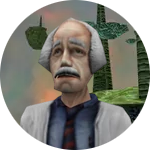
\includegraphics[width=3cm]{opening/resources/about/coomer.png} & \vspace{-0.5mm} {\large \bf \thesisTutor} 
        \hfill
        \href{https://orcid.org/}{  % Link to your orcid
            \icon{\faOrcid}{10}{orcid-green}
        }
        \href{https://www.linkedin.com/}{  % Link to your linkedin
            \icon{\faLinkedinIn}{10}{linkedin-blue}
        }
        \href{https://github.com/}{  % Link to your github
            \icon{\faGithub}{10}{github-black}
        }
        % \href{https://twitter.com/}{  % Link to your twitter
        %     \icon{\faTwitter}{10}{twitter-blue}
        % }
        \href{mailto:example@domain.org}{  % Your E-mail
            \icon{\faEnvelope}{10}{email-red}
        }
        \href{https://t.me/}{  % Link to your telegram
            \icon{\faTelegramPlane}{10}{telegram-blue}
        }
        \vspace{2mm} 
        \newline What a big fish you've got yourself. Show off your tutor. Now that's a job well done. Lorem ipsum dolor sit amet, consectetur adipiscing elit. Integer tempus quis elit id sagittis. Cras tincidunt nisi at tellus luctus, et congue dolor posuere. Aliquam suscipit felis sit amet lacus ultrices aliquet. Sed sagittis ultrices nisi, vel elementum elit dignissim non. Fusce faucibus ex at massa ultrices elementum.
    \end{tabular}
    
\endgroup





%%%%%%%%%%%%%%%%%%%%%%%%%%%%%%%%%%%%%%%%%%%%%%%%%%%%%%%%%%%%%%%%%%%%%%%%%%%%%%%%%%%%%%%%%%%%
% how to cite this work

% Listings workaround to include the background in broken lines

% \begin{verbatimwrite}{cite.txt}
% @mastersthesis{citeKey,
%     author  = "(*@{\thesisAuthor}@*) and (*@{\thesisTutor}@*)",
%     title   = "(*@{\thesisTitle}@*)",
%     school  = "(*@{\thesisSchool}@*)",
%     year    = "(*@{\thesisYear}@*)",
%     month   = "(*@{\thesisMonth}@*)",
%     address = "(*@{\thesisAddress}@*)"
% }
% \end{verbatimwrite}


\begingroup

\vspace*{\fill}

\small
\setlength\tabcolsep{0pt}
\renewcommand*{\arraystretch}{1.2}
{\noindent\large  Cite this work:}

% \begin{mdframed}[backgroundcolor=listing-background,hidealllines=true]
\vspace*{2mm}
% \lstinputlisting[style=cite, nolol]{./cite.txt}

\newwrite\tempfile
\immediate\openout\tempfile=cite.txt
\immediate\write\tempfile{%
@mastersthesis{citeKey,^^J
author  = "\thesisAuthor \space and \thesisTutor",^^J
title   = "\thesisTitle",^^J
school  = "\thesisSchool",^^J
year    = "\thesisYear",^^J
month   = "\thesisMonth",^^J
address = "\thesisAddress",^^J
type = "\thesisType"^^J
}
}
\immediate\closeout\tempfile

% Does not work because escapes are inside strings
% \begin{minted}{bibtex}
% @mastersthesis{citeKey,
%     author  = "¢{\thesisAuthor}¢ and ¢{\thesisTutor}¢",
%     title   = "¢{\thesisTitle}¢",
%     school  = "¢{\thesisSchool}¢",
%     year    = "¢{\thesisYear}¢",
%     month   = "¢{\thesisMonth}¢",
%     address = "¢{\thesisAddress}¢"
% }
% \end{minted}

\inputminted[style=algol_nu]{bibtex}{./cite.txt}
% \end{mdframed}


\endgroup


% Abstract
% 
%            ,,                                        
%          `7MM            _.o9                                
%            MM                                             
%  ,6"Yb.    MM  ,p6"bo   ,6"Yb.  M"""MMV  ,6"Yb.  `7Mb,od8 
% 8)   MM    MM 6M'  OO  8)   MM  '  AMV  8)   MM    MM' "' 
%  ,pm9MM    MM 8M        ,pm9MM    AMV    ,pm9MM    MM     
% 8M   MM    MM YM.    , 8M   MM   AMV  , 8M   MM    MM     
% `Moo9^Yo..JMML.YMbmd'  `Moo9^Yo.AMMmmmM `Moo9^Yo..JMML.   
% 
% 
% Free and Open-Source template for academic works
% https://github.com/dpmj/alcazar

\newpage

\clearpage
\cleardoublepage
\phantomsection

\pagestyle{empty}

\phantomsection
\addcontentsline{toc}{chapter}{Abstract}

{\noindent \large \textbf{\thesisTitle}}\\

{\noindent \textbf{\textsc{Keywords:}}}

{\noindent \thesisKeywords}\\


{\noindent \textbf{\textsc{Abstract:}}}

\noindent Abstract in the same language as the main text. Lorem ipsum dolor sit amet, consectetur adipiscing elit. Integer tempus quis elit id sagittis. Cras tincidunt nisi at tellus luctus, et congue dolor posuere. Aliquam suscipit felis sit amet lacus ultrices aliquet. Sed sagittis ultrices nisi, vel elementum elit dignissim non. Fusce faucibus ex at massa ultrices elementum. Nullam ullamcorper lorem sit amet facilisis cursus. Suspendisse non erat non justo porta placerat. Morbi porttitor dictum molestie. Sed vitae iaculis libero. Suspendisse in gravida lacus, tempor ultrices nibh. Nam consequat scelerisque porttitor.

Nulla elementum orci in dolor dapibus, ac facilisis sem ultrices. Nullam eleifend id eros sed luctus. Maecenas arcu ipsum, scelerisque id lorem in, placerat posuere tellus. Etiam gravida velit sed arcu viverra dapibus. Mauris vitae augue dapibus, molestie justo eget, condimentum ipsum. Nulla tristique mi eget semper luctus. Etiam commodo vestibulum vulputate. Etiam quis sapien dolor. Nunc tristique eu lacus quis ullamcorper. Sed volutpat rutrum vehicula. Donec nunc nisl, suscipit in faucibus vitae, tristique eu risus. Nulla facilisis augue eget interdum rutrum. Aliquam sem nunc, fermentum sed urna ac, faucibus interdum nisi.

Proin a condimentum nibh. Praesent vulputate tellus vel metus rutrum, non luctus mi sollicitudin. Nam ac tellus ut eros sollicitudin luctus at ac mi. Vestibulum mollis nec nisi a laoreet. Proin neque tortor, placerat nec suscipit sit amet, ullamcorper in sem. Fusce faucibus ultrices cursus. Maecenas scelerisque mauris diam, at volutpat nisi porta vitae. Sed at ipsum et leo cursus varius eu eu lectus. Class aptent taciti sociosqu ad litora torquent per conubia nostra, per inceptos himenaeos. Ut felis ipsum, imperdiet rhoncus orci ac, consectetur luctus nisl. Cras aliquet elementum tellus ullamcorper malesuada. Integer purus est, pharetra eu ullamcorper quis, imperdiet non turpis.

In vestibulum faucibus ligula eget blandit. Donec eget cursus risus, quis suscipit justo. Curabitur efficitur, dolor nec pulvinar pellentesque, lectus eros hendrerit nisi, in aliquet erat nunc non ipsum. Curabitur felis nunc, viverra nec quam ultrices, suscipit condimentum nibh. Nam faucibus felis hendrerit imperdiet maximus. Curabitur tincidunt porttitor lectus quis feugiat. Sed imperdiet bibendum mi.

Nullam quis lacus vel ante feugiat efficitur id ut quam. Pellentesque commodo elit nec urna gravida maximus. Suspendisse ut risus eu ipsum porta porta ac et orci. Donec dictum ligula sodales, euismod est sed, semper libero. In blandit, nulla et elementum pharetra, mi nunc sagittis tellus, sit amet scelerisque magna elit ac sapien. Curabitur ipsum dui, pretium a maximus id, varius gravida nisl. Sed vitae mattis elit, vitae hendrerit lorem. 



%% ADDITIONAL LANGUAGES
% Translate your title and keywords to match the language


\newpage

\clearpage
\cleardoublepage
\phantomsection

\pagestyle{empty}

{\noindent \large \textbf{\thesisTitle}}\\

{\noindent \textbf{\textsc{Palabras clave:}}}

{\noindent \thesisKeywords}\\


{\noindent \textbf{\textsc{Resumen:}}}

\noindent Resumen en un idioma diferente - Abstract in a different language.
Lorem ipsum dolor sit amet, consectetur adipiscing elit. Integer tempus quis elit id sagittis. Cras tincidunt nisi at tellus luctus, et congue dolor posuere. Aliquam suscipit felis sit amet lacus ultrices aliquet. Sed sagittis ultrices nisi, vel elementum elit dignissim non. Fusce faucibus ex at massa ultrices elementum. Nullam ullamcorper lorem sit amet facilisis cursus. Suspendisse non erat non justo porta placerat. Morbi porttitor dictum molestie. Sed vitae iaculis libero. Suspendisse in gravida lacus, tempor ultrices nibh. Nam consequat scelerisque porttitor.

Nulla elementum orci in dolor dapibus, ac facilisis sem ultrices. Nullam eleifend id eros sed luctus. Maecenas arcu ipsum, scelerisque id lorem in, placerat posuere tellus. Etiam gravida velit sed arcu viverra dapibus. Mauris vitae augue dapibus, molestie justo eget, condimentum ipsum. Nulla tristique mi eget semper luctus. Etiam commodo vestibulum vulputate. Etiam quis sapien dolor. Nunc tristique eu lacus quis ullamcorper. Sed volutpat rutrum vehicula. Donec nunc nisl, suscipit in faucibus vitae, tristique eu risus. Nulla facilisis augue eget interdum rutrum. Aliquam sem nunc, fermentum sed urna ac, faucibus interdum nisi.

Proin a condimentum nibh. Praesent vulputate tellus vel metus rutrum, non luctus mi sollicitudin. Nam ac tellus ut eros sollicitudin luctus at ac mi. Vestibulum mollis nec nisi a laoreet. Proin neque tortor, placerat nec suscipit sit amet, ullamcorper in sem. Fusce faucibus ultrices cursus. Maecenas scelerisque mauris diam, at volutpat nisi porta vitae. Sed at ipsum et leo cursus varius eu eu lectus. Class aptent taciti sociosqu ad litora torquent per conubia nostra, per inceptos himenaeos. Ut felis ipsum, imperdiet rhoncus orci ac, consectetur luctus nisl. Cras aliquet elementum tellus ullamcorper malesuada. Integer purus est, pharetra eu ullamcorper quis, imperdiet non turpis.

In vestibulum faucibus ligula eget blandit. Donec eget cursus risus, quis suscipit justo. Curabitur efficitur, dolor nec pulvinar pellentesque, lectus eros hendrerit nisi, in aliquet erat nunc non ipsum. Curabitur felis nunc, viverra nec quam ultrices, suscipit condimentum nibh. Nam faucibus felis hendrerit imperdiet maximus. Curabitur tincidunt porttitor lectus quis feugiat. Sed imperdiet bibendum mi.

Nullam quis lacus vel ante feugiat efficitur id ut quam. Pellentesque commodo elit nec urna gravida maximus. Suspendisse ut risus eu ipsum porta porta ac et orci. Donec dictum ligula sodales, euismod est sed, semper libero. In blandit, nulla et elementum pharetra, mi nunc sagittis tellus, sit amet scelerisque magna elit ac sapien. Curabitur ipsum dui, pretium a maximus id, varius gravida nisl. Sed vitae mattis elit, vitae hendrerit lorem. 



% Dedication
% To whom do you dedicate the thesis? Or maybe include a quote, poem, etc. Free space for yourself.
% Delete if you are too manly for these things
% 
%            ,,                                        
%          `7MM            _.o9                                
%            MM                                             
%  ,6"Yb.    MM  ,p6"bo   ,6"Yb.  M"""MMV  ,6"Yb.  `7Mb,od8 
% 8)   MM    MM 6M'  OO  8)   MM  '  AMV  8)   MM    MM' "' 
%  ,pm9MM    MM 8M        ,pm9MM    AMV    ,pm9MM    MM     
% 8M   MM    MM YM.    , 8M   MM   AMV  , 8M   MM    MM     
% `Moo9^Yo..JMML.YMbmd'  `Moo9^Yo.AMMmmmM `Moo9^Yo..JMML.   
% 
% 
% Free and Open-Source template for academic works
% https://github.com/dpmj/alcazar

\newpage

\clearpage
\cleardoublepage
\phantomsection

\pagestyle{empty}

\phantomsection
\addcontentsline{toc}{chapter}{Dedication}



\vspace*{\fill}

\begin{flushright}

\textit{\large
\noindent ``Y así, mi señor, es como sabemos que\\
la Tierra tiene forma de plátano''\\ 
}

\vspace{0.5cm}

\textbf{Sir Bedevere el Sabio}\\

\vspace{0.3cm}

Interpretado por \textsc{Terry Jones}\\

\vspace{0.2cm}

{
\noindent En \textit{Monty Python y los caballeros\\
de la mesa cuadrada,} 1975\\
}

\vspace{2cm}
\end{flushright}



\vspace*{\fill}

% Acknowledgements
% 
%            ,,                                        
%          `7MM            _.o9                                
%            MM                                             
%  ,6"Yb.    MM  ,p6"bo   ,6"Yb.  M"""MMV  ,6"Yb.  `7Mb,od8 
% 8)   MM    MM 6M'  OO  8)   MM  '  AMV  8)   MM    MM' "' 
%  ,pm9MM    MM 8M        ,pm9MM    AMV    ,pm9MM    MM     
% 8M   MM    MM YM.    , 8M   MM   AMV  , 8M   MM    MM     
% `Moo9^Yo..JMML.YMbmd'  `Moo9^Yo.AMMmmmM `Moo9^Yo..JMML.   
% 
% 
% Free and Open-Source template for academic works
% https://github.com/dpmj/alcazar


% Add here your Acknowledgements. 
% This section is pretty free: free format, in one or various languages, etc.


\newpage
\thispagestyle{empty}

\clearpage
\cleardoublepage
\phantomsection

\pagestyle{plain}

\phantomsection
\addcontentsline{toc}{chapter}{Acknowledgements}


\vspace*{\fill}

\begin{center}
    \large \textbf{\textsc{Acknowledgements}}
\end{center}

Lorem ipsum dolor sit amet, consectetur adipiscing elit. Integer tempus quis elit id sagittis. Cras tincidunt nisi at tellus luctus, et congue dolor posuere. Aliquam suscipit felis sit amet lacus ultrices aliquet. Sed sagittis ultrices nisi, vel elementum elit dignissim non. Fusce faucibus ex at massa ultrices elementum. Nullam ullamcorper lorem sit amet facilisis cursus. Suspendisse non erat non justo porta placerat. Morbi porttitor dictum molestie. Sed vitae iaculis libero. Suspendisse in gravida lacus, tempor ultrices nibh. Nam consequat scelerisque porttitor.

Nulla elementum orci in dolor dapibus, ac facilisis sem ultrices. Nullam eleifend id eros sed luctus. Maecenas arcu ipsum, scelerisque id lorem in, placerat posuere tellus. Etiam gravida velit sed arcu viverra dapibus. Mauris vitae augue dapibus, molestie justo eget, condimentum ipsum. Nulla tristique mi eget semper luctus. Etiam commodo vestibulum vulputate. 

Etiam quis sapien dolor. Nunc tristique eu lacus quis ullamcorper. Sed volutpat rutrum vehicula. Donec nunc nisl, suscipit in faucibus vitae, tristique eu risus. Nulla facilisis augue eget interdum rutrum. Aliquam sem nunc, fermentum sed urna ac, faucibus interdum nisi.

\vspace*{1cm}

\vspace*{\fill}





% TABLES OF CONTENTS

\begingroup

    \renewcommand{\baselinestretch}{0.3}\normalsize  % Comprime space used by TOC
    
    % List of Contents
    \tableofcontents
    \addcontentsline{toc}{chapter}{Table of contents}
    
    % List of Figures
    \listoffigures
    \addcontentsline{toc}{chapter}{List of figures}
    
    % List of Tables
    \listoftables
    \addcontentsline{toc}{chapter}{List of tables}
    
    % List of Listings
    {
        % This particular toc uses shorter spacing for some reason

        \renewcommand{\baselinestretch}{1.2}\normalsize
        
        \listof{lstlisting}{Code listings} % \lstlistoflistings
        \addcontentsline{toc}{chapter}{Code listings}
    }
    
\endgroup

% END OPENING






% Glossary and acronyms
% 
%            ,,                                        
%          `7MM            _.o9                                
%            MM                                             
%  ,6"Yb.    MM  ,p6"bo   ,6"Yb.  M"""MMV  ,6"Yb.  `7Mb,od8 
% 8)   MM    MM 6M'  OO  8)   MM  '  AMV  8)   MM    MM' "' 
%  ,pm9MM    MM 8M        ,pm9MM    AMV    ,pm9MM    MM     
% 8M   MM    MM YM.    , 8M   MM   AMV  , 8M   MM    MM     
% `Moo9^Yo..JMML.YMbmd'  `Moo9^Yo.AMMmmmM `Moo9^Yo..JMML.   
% 
% 
% Free and Open-Source template for academic works
% https://github.com/dpmj/alcazar


%%%%%%%%%%%%%%%%%%%%%%%%%%%%%%%%%%%%%%%%%%%%%%%%%%%%%%%%%%%%%%%%%%%%%%%%%%%%%%%%%%%%%%%%%%%%
% GLOSSARY


\clearpage
\cleardoublepage
\phantomsection

{
    \footnotesize
    \printglossaries
}


% Chapters - main text
% 
%            ,,                                        
%          `7MM            _.o9                                
%            MM                                             
%  ,6"Yb.    MM  ,p6"bo   ,6"Yb.  M"""MMV  ,6"Yb.  `7Mb,od8 
% 8)   MM    MM 6M'  OO  8)   MM  '  AMV  8)   MM    MM' "' 
%  ,pm9MM    MM 8M        ,pm9MM    AMV    ,pm9MM    MM     
% 8M   MM    MM YM.    , 8M   MM   AMV  , 8M   MM    MM     
% `Moo9^Yo..JMML.YMbmd'  `Moo9^Yo.AMMmmmM `Moo9^Yo..JMML.   
% 
% 
% Free and Open-Source template for academic works
% https://github.com/dpmj/alcazar


% Start standard numbering and page style

\clearpage
\phantomsection

\pagestyle{chapters}
\pagenumbering{arabic}
\setcounter{page}{1}

\input{text/chapters/1.Introduction}
\input{text/chapters/2.LitReview}
\input{text/chapters/3.ResearchQuestions}
\input{text/chapters/4.Methods}
\input{text/chapters/5.Progress}
\input{text/chapters/6.JournalPlan}
\input{text/chapters/7.Gantt}

% Bibliography
% 
%            ,,                                        
%          `7MM            _.o9                                
%            MM                                             
%  ,6"Yb.    MM  ,p6"bo   ,6"Yb.  M"""MMV  ,6"Yb.  `7Mb,od8 
% 8)   MM    MM 6M'  OO  8)   MM  '  AMV  8)   MM    MM' "' 
%  ,pm9MM    MM 8M        ,pm9MM    AMV    ,pm9MM    MM     
% 8M   MM    MM YM.    , 8M   MM   AMV  , 8M   MM    MM     
% `Moo9^Yo..JMML.YMbmd'  `Moo9^Yo.AMMmmmM `Moo9^Yo..JMML.   
% 
% 
% Free and Open-Source template for academic works
% https://github.com/dpmj/alcazar


\clearpage
\cleardoublepage

\pagestyle{biblio}

\phantomsection
\addcontentsline{toc}{chapter}{Bibliography}

{
    \renewcommand{\UrlFont}{\ttfamily\fontsize{9}{9}\selectfont}  
    % Smaller URLs (USE FOR IBM PLEX MONO ONLY)
    
    \footnotesize  % Compress space used by bibliography

    % For bibtex bibliography
    % \bibliographystyle{ieeetr}
    % \bibliography{bibliography/references}

    % Multi-column bibliography 
    % For biblatex bibliography
    \begin{multicols}{2}[\printbibheading]
        \renewcommand{\baselinestretch}{0.95}
        \AtNextBibliography{\footnotesize \pagestyle{biblio}}
        \printbibliography[heading=none]  
    \end{multicols}

}


% Addendum - secondary text
% 
%            ,,                                        
%          `7MM            _.o9                                
%            MM                                             
%  ,6"Yb.    MM  ,p6"bo   ,6"Yb.  M"""MMV  ,6"Yb.  `7Mb,od8 
% 8)   MM    MM 6M'  OO  8)   MM  '  AMV  8)   MM    MM' "' 
%  ,pm9MM    MM 8M        ,pm9MM    AMV    ,pm9MM    MM     
% 8M   MM    MM YM.    , 8M   MM   AMV  , 8M   MM    MM     
% `Moo9^Yo..JMML.YMbmd'  `Moo9^Yo.AMMmmmM `Moo9^Yo..JMML.   
% 
% 
% Free and Open-Source template for academic works
% https://github.com/dpmj/alcazar



\clearpage
\cleardoublepage


\begin{appendices}

    \pagestyle{addenda}

    \renewcommand\chaptername{Appendix}  
    % Change name of the chapters
    % This is due to a conflict with titlesec


    % 
%            ,,                                        
%          `7MM            _.o9                                
%            MM                                             
%  ,6"Yb.    MM  ,p6"bo   ,6"Yb.  M"""MMV  ,6"Yb.  `7Mb,od8 
% 8)   MM    MM 6M'  OO  8)   MM  '  AMV  8)   MM    MM' "' 
%  ,pm9MM    MM 8M        ,pm9MM    AMV    ,pm9MM    MM     
% 8M   MM    MM YM.    , 8M   MM   AMV  , 8M   MM    MM     
% `Moo9^Yo..JMML.YMbmd'  `Moo9^Yo.AMMmmmM `Moo9^Yo..JMML.   
% 
% 
% Free and Open-Source template for academic works
% https://github.com/dpmj/alcazar


% Example of an appendix


\chapter{Something you put a lot of effort into but which was vaguely related to the main content}


\section{Praesent vulputate tellus vel metus rutrum}


Lorem ipsum dolor sit amet, consectetur adipiscing elit. Integer tempus quis elit id sagittis. Cras tincidunt nisi at tellus luctus, et congue dolor posuere. Aliquam suscipit felis sit amet lacus ultrices aliquet. Sed sagittis ultrices nisi, vel elementum elit dignissim non. Fusce faucibus ex at massa ultrices elementum. Nullam ullamcorper lorem sit amet facilisis cursus. Suspendisse non erat non justo porta placerat. Morbi porttitor dictum molestie. Sed vitae iaculis libero. Suspendisse in gravida lacus, tempor ultrices nibh. Nam consequat scelerisque porttitor \cite{europa_rohs, europa_ce}.


\subsection{Faucibus interdum nisi}

Nulla elementum orci in dolor dapibus, ac facilisis sem ultrices. Nullam eleifend id eros sed luctus. Maecenas arcu ipsum, scelerisque id lorem in, placerat posuere tellus \cite{proceedings_piezo}. Etiam gravida velit sed arcu viverra dapibus. Mauris vitae augue dapibus, molestie justo eget, condimentum ipsum. Nulla tristique mi eget semper luctus. Etiam commodo vestibulum vulputate. Etiam quis sapien dolor. Nunc tristique eu lacus quis ullamcorper. Sed volutpat rutrum vehicula. Donec nunc nisl, suscipit in faucibus vitae, tristique eu risus. \glsname{GNU} nulla facilisis augue eget interdum rutrum. Aliquam sem nunc, fermentum sed urna ac, faucibus interdum nisi.


\subsection{Praesent vulputate tellus vel metus rutrum}

Proin a condimentum nibh. Praesent vulputate tellus vel metus rutrum, non luctus mi sollicitudin. Nam ac tellus ut eros sollicitudin luctus at ac mi. Vestibulum mollis nec nisi a laoreet. Proin neque tortor, placerat nec suscipit sit amet, ullamcorper in sem. Fusce faucibus ultrices cursus. Maecenas scelerisque mauris diam, at volutpat nisi porta vitae. 

Sed at ipsum et leo cursus varius eu eu lectus. Class aptent taciti sociosqu ad litora torquent per conubia nostra, per inceptos himenaeos. 

Ut felis ipsum, imperdiet rhoncus orci ac, consectetur luctus nisl. Cras aliquet elementum tellus ullamcorper malesuada. Integer purus est, pharetra eu ullamcorper quis, imperdiet non turpis. \cite{SOFTWARE_ENGINEERING_9}




\begin{figure}[!hp]
    \centering
    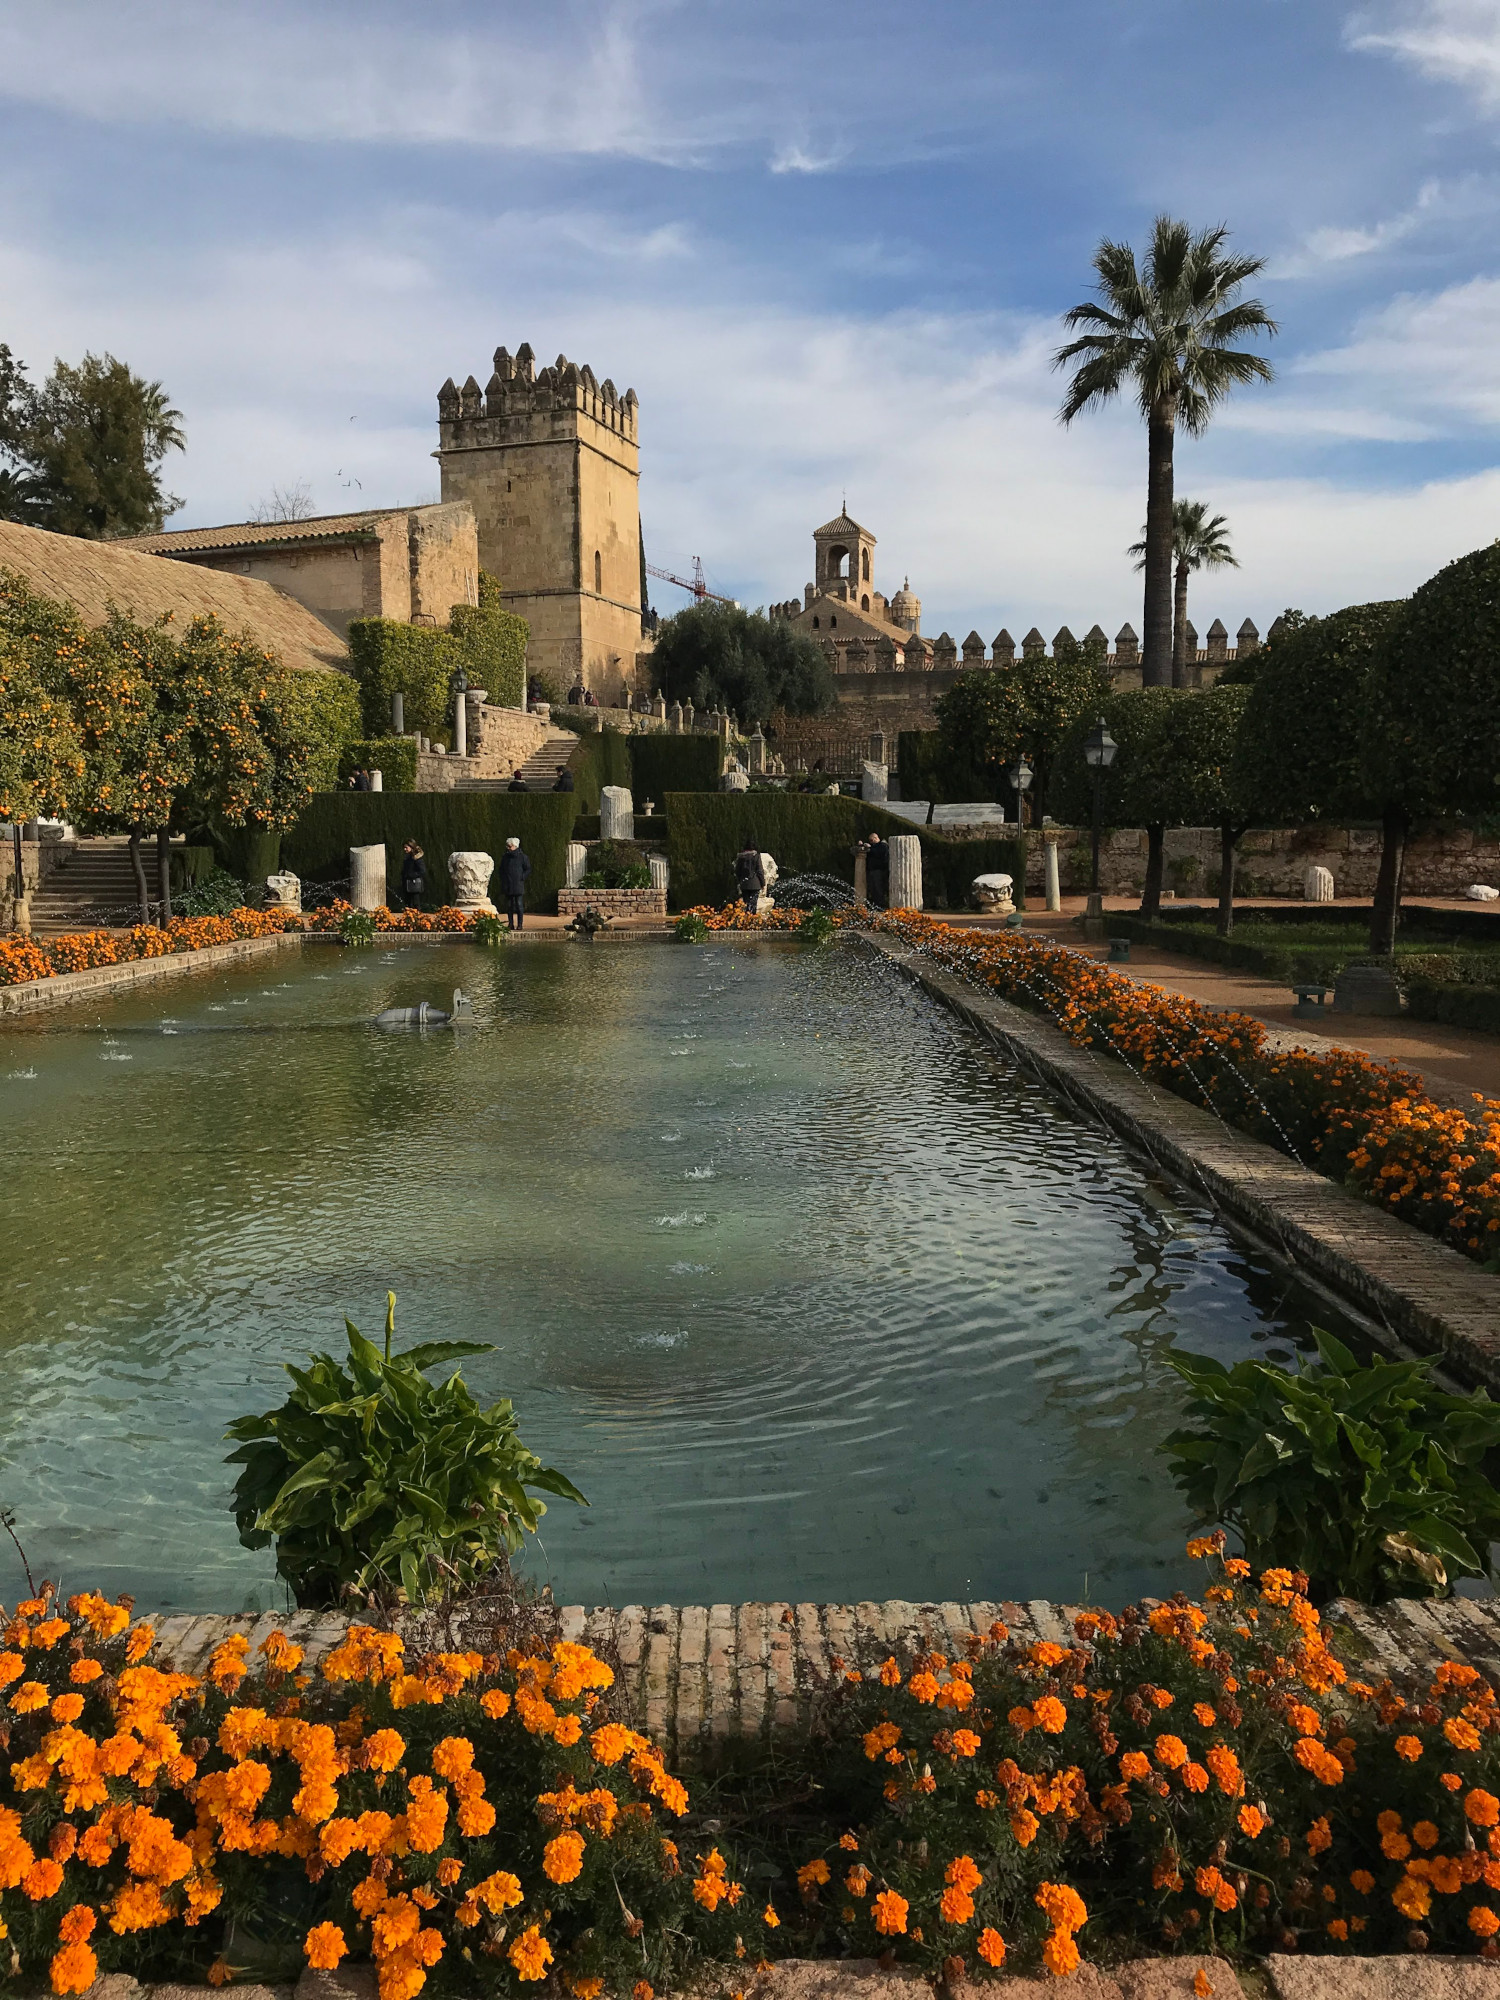
\includegraphics[width=\linewidth]{figures/examples/Alcazar_Cordoba.jpg}
    \caption[Alcázar de los reyes cristianos, Córdoba.]{Alcázar de los reyes cristianos, Córdoba. \href{https://es.wikipedia.org/wiki/Archivo:Alcazar_Cordoba.jpg}{Ahura klik}.}
    \label{fig:apxA:cordoba}
\end{figure}



In vestibulum faucibus ligula eget blandit. Donec eget cursus risus, quis suscipit justo. Curabitur efficitur, dolor nec pulvinar pellentesque, lectus eros hendrerit nisi, in aliquet erat nunc non ipsum. Curabitur felis nunc, viverra nec quam ultrices, suscipit condimentum nibh. Nam faucibus felis hendrerit imperdiet maximus. Curabitur tincidunt porttitor lectus quis feugiat. Sed imperdiet bibendum mi.

\begin{description}
    \item[Nullam quis lacus] vel ante feugiat efficitur id ut quam. Pellentesque commodo elit nec urna gravida maximus. Suspendisse ut risus eu ipsum porta porta ac et orci. Donec dictum ligula sodales, euismod est sed, semper libero \glsname{fiducial}. 
    \item[In blandit], nulla et elementum pharetra, mi nunc sagittis tellus, sit amet scelerisque magna elit ac sapien. Curabitur ipsum dui, pretium a maximus id, varius gravida nisl. Sed vitae mattis elit, vitae hendrerit lorem \cite{IEEE315}.
\end{description}

\subsubsection{Lorem ipsum dolor sit amet, consectetur adipiscing elit}

Integer tempus quis elit id sagittis. Cras tincidunt nisi at tellus luctus, et congue dolor posuere. Aliquam suscipit felis sit amet lacus ultrices aliquet. Sed sagittis ultrices nisi, vel elementum elit dignissim non. 

\subsubsection{Fusce faucibus ex at massa ultrices elementum}

Nullam ullamcorper lorem sit amet facilisis cursus. Suspendisse non erat non justo porta placerat. Morbi porttitor dictum molestie. Sed vitae iaculis libero. Suspendisse in gravida lacus, tempor ultrices nibh. Nam consequat scelerisque porttitor.

\section{Nulla elementum orci in dolor dapibus}

Nulla elementum orci in dolor dapibus, ac facilisis sem ultrices. Nullam eleifend id eros sed luctus. Maecenas arcu ipsum, scelerisque id lorem in, placerat posuere tellus. Etiam gravida velit sed arcu viverra dapibus. Mauris vitae augue dapibus, molestie justo eget, condimentum ipsum. Nulla tristique mi eget semper luctus. Etiam commodo vestibulum vulputate. Etiam quis sapien dolor. Nunc tristique eu lacus quis ullamcorper. Sed volutpat rutrum vehicula. Donec nunc nisl, suscipit in faucibus vitae, tristique eu risus. Nulla facilisis augue eget interdum rutrum. Aliquam sem nunc, fermentum sed urna ac, faucibus interdum nisi.

\subsection{Non luctus mi sollicitudin}

Nam ac tellus ut eros sollicitudin luctus at ac mi. Vestibulum mollis nec nisi a laoreet. Proin neque tortor, placerat nec suscipit sit amet, ullamcorper in sem. Fusce faucibus ultrices cursus. Maecenas scelerisque mauris diam, at volutpat nisi porta vitae. Sed at ipsum et leo cursus varius eu eu lectus. Class aptent taciti sociosqu ad litora torquent per conubia nostra, per inceptos himenaeos. Ut felis ipsum, imperdiet rhoncus orci ac, consectetur luctus nisl. Cras aliquet elementum tellus ullamcorper malesuada. Integer purus est, pharetra eu ullamcorper quis, imperdiet non turpis.

In vestibulum faucibus ligula eget blandit. Donec eget cursus risus, quis suscipit justo. Curabitur efficitur, dolor nec pulvinar pellentesque, lectus eros hendrerit nisi, in aliquet erat nunc non ipsum. Curabitur felis nunc, viverra nec quam ultrices, suscipit condimentum nibh. Nam faucibus felis hendrerit imperdiet maximus. Curabitur tincidunt porttitor lectus quis feugiat. Sed imperdiet bibendum mi.

\subsubsection{Nullam quis lacus vel ante feugiat}

Nullam quis lacus vel ante feugiat efficitur id ut quam. Pellentesque commodo elit nec urna gravida maximus. Suspendisse ut risus eu ipsum porta porta ac et orci. Donec dictum ligula sodales, euismod est sed, semper libero. In blandit, nulla et elementum pharetra, mi nunc sagittis tellus, sit amet scelerisque magna elit ac sapien. Curabitur ipsum dui, pretium a maximus id, varius gravida nisl. Sed vitae mattis elit, vitae hendrerit lorem. 


\begin{lstlisting}[caption={Some Python Code \cite{esp32_devkit_reference_design}}, language=PythonPlus, style=ColorEX]
"""
Some interesting python code 
Blah Blah Blah
"""

import numpy as np
from matplotlib import pyplot as plt
from numpy.polynomial import Polynomial as Poly

plt.rcParams["font.family"] = "Libertinus Serif"
plt.rcParams['font.size'] = 14
plt.rcParams['mathtext.fontset'] = 'custom'
plt.rcParams['mathtext.rm'] = 'Libertinus Serif'
plt.rcParams['mathtext.it'] = 'Libertinus Serif:italic'
plt.rcParams['mathtext.bf'] = 'Libertinus Serif:bold'

R510 = 508.3  # Ohms
V5 = 5.018  # Volts

# Open files

nmos_vgs, nmos_vr = np.loadtxt('nmos_ids_vgs.csv', delimiter='\t', unpack=True, skiprows=1)
nmos_sim_vgs, nmos_sim_ids = np.loadtxt('CIC_P0_NMOS_ids_vgs_5.txt', delimiter='\t', unpack=True, skiprows=1)

# Do thingies

nmos_ids = nmos_vr / R510  # Current in resistor
p = Poly.fit(nmos_vgs, nmos_ids, 1)  # Tendency line
print(f"f(x) = {p:unicode}")

# Plot stuff

fig0, ax0 = plt.subplots(figsize=[12, 6])
x = np.linspace(0, 6, 100)

plt.plot(nmos_vgs, nmos_ids, linestyle='none', marker=".", label='Experimental')
plt.plot(nmos_sim_vgs, nmos_sim_ids, linestyle='dashdot', label='Simulation')
plt.plot(x, p(x), linestyle='dashed', label='Tendency')

ax0.grid(True, which='major', color='#DDDDDD', linestyle='-', linewidth=0.6)
ax0.grid(True, which='minor', color='#DDDDDD', linestyle=':', linewidth=0.6)
ax0.minorticks_on()

ax0.legend()

plt.title(r'NMOS, curve $I_{DS}$ / $V_{GS}$')
plt.xlabel(r'$V_{GS}$ (V)')
plt.ylabel(r'$I_{DS}$ (A)')

plt.xlim([0, 6])

# Dont forget to save

plt.savefig("nmos_vgs_ids.pdf")
\end{lstlisting}


    % 
%            ,,                                        
%          `7MM            _.o9                                
%            MM                                             
%  ,6"Yb.    MM  ,p6"bo   ,6"Yb.  M"""MMV  ,6"Yb.  `7Mb,od8 
% 8)   MM    MM 6M'  OO  8)   MM  '  AMV  8)   MM    MM' "' 
%  ,pm9MM    MM 8M        ,pm9MM    AMV    ,pm9MM    MM     
% 8M   MM    MM YM.    , 8M   MM   AMV  , 8M   MM    MM     
% `Moo9^Yo..JMML.YMbmd'  `Moo9^Yo.AMMmmmM `Moo9^Yo..JMML.   
% 
% 
% Free and Open-Source template for academic works
% https://github.com/dpmj/alcazar


% Example of another appendix




\chapter{A long table of things}

Lorem ipsum dolor sit amet, consectetur adipiscing elit. Integer tempus quis elit id sagittis. Cras tincidunt nisi at tellus luctus, et congue dolor posuere. Aliquam suscipit felis sit amet lacus ultrices aliquet. Sed sagittis ultrices nisi, vel elementum elit dignissim non. Fusce faucibus ex at massa ultrices elementum. Nullam ullamcorper lorem sit amet facilisis cursus. Suspendisse non erat non justo porta placerat. Morbi porttitor dictum molestie. Sed vitae iaculis libero. Suspendisse in gravida lacus, tempor ultrices nibh. Nam consequat scelerisque porttitor \footnote{And if you can believe it, It's a Friday once again!}.

Nulla elementum orci in dolor dapibus, ac facilisis sem ultrices. Nullam eleifend id eros sed luctus. Maecenas arcu ipsum, scelerisque id lorem in, placerat posuere tellus. 

Etiam gravida velit sed arcu viverra dapibus. Mauris vitae augue dapibus, molestie justo eget, condimentum ipsum. Nulla tristique mi eget semper luctus \autoref{tab:predecesoras-1}. 


\begin{landscape}
    \begin{table}[p]
    \scriptsize
    \centering
    \renewcommand{\arraystretch}{1.2}
    
    \caption{Example of a long landscape table.}
    \label{tab:predecesoras-1}
    \begin{tabular}{|l|l|p{5.5cm}|l|l|l|l|l|p{5.5cm}|}
    \hline
    \textbf{Nº} & \textbf{EDT} & \textbf{Nombre de tarea} & \textbf{Trabajo} & \textbf{Duración} & \textbf{Predecesoras} & \textbf{Comienzo} & \textbf{Fin} & \textbf{Recursos} \\ \hline\hline
    \textbf{1} & \textbf{1} & \textbf{Dirección del proyecto} & 4 días & 4 días &  & lun 03/07/23 & jue 06/07/23 &  \\ \hline
    2 & 1.1 & Reunión inicial de planificación con el cliente & 3 días & 3 días &  & lun 03/07/23 & mié 05/07/23 & Ana Torres;Carla Aguilar;Diego Ortiz;Lucía   Castro;Martina Martinez;Pablo Gómez;Rodrigo García \\ \hline
    3 & 1.2 & Reparto de tareas a los trabajadores & 1 día & 1 día & 1.1 & jue 06/07/23 & jue 06/07/23 & Ana Torres \\ \hline
    \textbf{4} & \textbf{2} & \textbf{Estudio de la viabilidad del despliegue} & \textbf{27 días} & \textbf{9,67 días} & \textbf{} & \textbf{vie 07/07/23} & \textbf{jue 20/07/23} & \textbf{} \\ \hline
    5 & 2.1 & Estudio de la orografía & 5 días & 1,67 días & 1.2 & vie 07/07/23 & lun 10/07/23 & Rodrigo García;Paloma Cuesta;Ramón García \\ \hline
    6 & 2.2 & Estudio del emplazamiento de las antenas del   radioenlace y balance de potencias & 4 días & 1,33 días & 2.1 & mié 12/07/23 & jue 13/07/23 & Rodrigo García;Paloma Cuesta;Ramón García \\ \hline
    7 & 2.3 & Estudio del emplazamiento de las estaciones   base y radio de cobertura & 4 días & 1,33 días & 2.1 & jue 13/07/23 & vie 14/07/23 & Rodrigo García;Paloma Cuesta;Ramón García \\ \hline
    8 & 2.4 & Estudio de la magnitud del tráfico & 3 días & 1 día & 1.2 & lun 10/07/23 & mar 11/07/23 & Rodrigo García;Paloma Cuesta;Ramón García \\ \hline
    9 & 2.5 & Revisión de la normativa & 2 días & 0,67 días & 1.2 & mar 11/07/23 & mié 12/07/23 & Rodrigo García;Paloma Cuesta;Ramón García \\ \hline
    10 & 2.6 & Establecimiento de los requisitos técnicos & 5 días & 1,67 días & 2.1;2.2;2.3;2.4;2.5 & lun 17/07/23 & mar 18/07/23 & Rodrigo García;Paloma Cuesta;Ramón García \\ \hline
    11 & 2.7 & Establecimiento de un presupuesto temprano & 4 días & 2 días & 2.6 & mar 18/07/23 & jue 20/07/23 & Ana Torres;Rodrigo García \\ \hline
    \textbf{12} & \textbf{3} & \textbf{Diseño del despliegue} & \textbf{41 días} & \textbf{14 días} & \textbf{} & \textbf{jue 20/07/23} & \textbf{mié 09/08/23} & \textbf{} \\ \hline
    13 & 3.1 & Diseño de la red & 29 días & 9,67 días &  & jue 20/07/23 & jue 03/08/23 &  \\ \hline
    14 & 3.1.1 & Diseño de las estaciones base de telefonía & 7 días & 9,67 días &  & jue 20/07/23 & jue 03/08/23 &  \\ \hline
    15 & 3.1.1.1 & Elección del emplazamiento físico & 5 días & 1,67 días & 2 & jue 20/07/23 & lun 24/07/23 & Rodrigo García;Paloma Cuesta;Ramón García \\ \hline
    16 & 3.1.1.2 & Diseño de la sectorización y el apuntado & 2 días & 0,67 días & 3.1.1.1 & mié 02/08/23 & jue 03/08/23 & Rodrigo García;Paloma Cuesta;Ramón García \\ \hline
    17 & 3.1.2 & Diseño de las estaciones base del radioenlace & 7 días & 2,33 días &  & lun 24/07/23 & mié 26/07/23 &  \\ \hline
    18 & 3.1.2.1 & Elección del emplazamiento físico & 5 días & 1,67 días & 2 & lun 24/07/23 & mar 25/07/23 & Rodrigo García;Paloma Cuesta;Ramón García \\ \hline
    19 & 3.1.2.2 & Diseño del apuntado & 2 días & 0,67 días & 3.1.2.1 & mié 26/07/23 & mié 26/07/23 & Rodrigo García;Paloma Cuesta;Ramón García \\ \hline
    20 & 3.1.3 & Diseño de la topología de red & 10 días & 3,33 días & 2 & mié 26/07/23 & lun 31/07/23 & Rodrigo García;Paloma Cuesta;Ramón García \\ \hline
    21 & 3.1.4 & Diseño de la gestión y separación del tráfico & 5 días & 1,67 días & 2 & mar 01/08/23 & mié 02/08/23 & Rodrigo García;Paloma Cuesta;Ramón García \\ \hline
    22 & 3.2 & Elección de equipos y componentes & 10 días & 3,33 días &  & jue 03/08/23 & mar 08/08/23 &  \\ \hline
    23 & 3.2.1 & Elección de los equipos de RF & 5 días & 1,67 días & 3.1 & jue 03/08/23 & vie 04/08/23 & Rodrigo García;Paloma Cuesta;Ramón García \\ \hline
    24 & 3.2.2 & Elección de los equipos de red & 5 días & 1,67 días & 3.1 & lun 07/08/23 & mar 08/08/23 & Rodrigo García;Paloma Cuesta;Ramón García \\ \hline
    25 & 3.3 & Elaboración del presupuesto base & 2 días & 1 día & 3.1;3.2 & mar 08/08/23 & mié 09/08/23 & Rodrigo García;Ana Torres \\ \hline
    \textbf{26} & \textbf{4} & \textbf{Despliegue físico} & \textbf{38 días} & \textbf{15,83 días} & \textbf{} & \textbf{mié 09/08/23} & \textbf{jue 31/08/23} & \textbf{} \\ \hline
    27 & 4.1 & Reunión de materiales & 4 días & 2 días & 3 & mié 09/08/23 & vie 11/08/23 & Diego Ortiz;Martina Martinez \\ \hline
    28 & 4.2 & Construcción & 15 días & 7,5 días &  & vie 11/08/23 & mié 23/08/23 &  \\ \hline
    29 & 4.2.1 & Estaciones de telefonía & 5 días & 2,5 días & 4.1 & vie 11/08/23 & mié 16/08/23 & Diego Ortiz;Martina Martinez \\ \hline
    \end{tabular}%
    \end{table}
\end{landscape}

\end{appendices}


% It's nice to say thanks. 
% 
%            ,,                                        
%          `7MM            _.o9                                
%            MM                                             
%  ,6"Yb.    MM  ,p6"bo   ,6"Yb.  M"""MMV  ,6"Yb.  `7Mb,od8 
% 8)   MM    MM 6M'  OO  8)   MM  '  AMV  8)   MM    MM' "' 
%  ,pm9MM    MM 8M        ,pm9MM    AMV    ,pm9MM    MM     
% 8M   MM    MM YM.    , 8M   MM   AMV  , 8M   MM    MM     
% `Moo9^Yo..JMML.YMbmd'  `Moo9^Yo.AMMmmmM `Moo9^Yo..JMML.   
% 
% 
% Free and Open-Source template for academic works
% https://github.com/dpmj/alcazar


% It's nice to say thanks


\newpage
\clearpage
\cleardoublepage

\thispagestyle{empty}

\vspace*{\fill}

\begin{center}
    \textbf{\large Thank you for reading this {\thesisType}.}
    \vspace{1cm}
\end{center}

\vspace*{\fill}


  % Optional: comment this line if you feel like it.


\end{document}

% END DOCUMENT
%%%%%%%%%%%%%%%%%%%%%%%%%%%%%%%%%%%%%%%%%%%%%%%%%%%%%%%%%%%%%%%%%%%%%%%%%%%%%%%%%%%%%%%%%%%%%%%%%%%%%%%%


